\documentclass[a4paper,12pt]{article}\usepackage[]{graphicx}\usepackage[]{color}
% maxwidth is the original width if it is less than linewidth
% otherwise use linewidth (to make sure the graphics do not exceed the margin)
\makeatletter
\def\maxwidth{ %
  \ifdim\Gin@nat@width>\linewidth
    \linewidth
  \else
    \Gin@nat@width
  \fi
}
\makeatother

\definecolor{fgcolor}{rgb}{0.345, 0.345, 0.345}
\newcommand{\hlnum}[1]{\textcolor[rgb]{0.686,0.059,0.569}{#1}}%
\newcommand{\hlstr}[1]{\textcolor[rgb]{0.192,0.494,0.8}{#1}}%
\newcommand{\hlcom}[1]{\textcolor[rgb]{0.678,0.584,0.686}{\textit{#1}}}%
\newcommand{\hlopt}[1]{\textcolor[rgb]{0,0,0}{#1}}%
\newcommand{\hlstd}[1]{\textcolor[rgb]{0.345,0.345,0.345}{#1}}%
\newcommand{\hlkwa}[1]{\textcolor[rgb]{0.161,0.373,0.58}{\textbf{#1}}}%
\newcommand{\hlkwb}[1]{\textcolor[rgb]{0.69,0.353,0.396}{#1}}%
\newcommand{\hlkwc}[1]{\textcolor[rgb]{0.333,0.667,0.333}{#1}}%
\newcommand{\hlkwd}[1]{\textcolor[rgb]{0.737,0.353,0.396}{\textbf{#1}}}%
\let\hlipl\hlkwb

\usepackage{framed}
\makeatletter
\newenvironment{kframe}{%
 \def\at@end@of@kframe{}%
 \ifinner\ifhmode%
  \def\at@end@of@kframe{\end{minipage}}%
  \begin{minipage}{\columnwidth}%
 \fi\fi%
 \def\FrameCommand##1{\hskip\@totalleftmargin \hskip-\fboxsep
 \colorbox{shadecolor}{##1}\hskip-\fboxsep
     % There is no \\@totalrightmargin, so:
     \hskip-\linewidth \hskip-\@totalleftmargin \hskip\columnwidth}%
 \MakeFramed {\advance\hsize-\width
   \@totalleftmargin\z@ \linewidth\hsize
   \@setminipage}}%
 {\par\unskip\endMakeFramed%
 \at@end@of@kframe}
\makeatother

\definecolor{shadecolor}{rgb}{.97, .97, .97}
\definecolor{messagecolor}{rgb}{0, 0, 0}
\definecolor{warningcolor}{rgb}{1, 0, 1}
\definecolor{errorcolor}{rgb}{1, 0, 0}
\newenvironment{knitrout}{}{} % an empty environment to be redefined in TeX

\usepackage{alltt}

% Packages
\usepackage{booktabs}
\usepackage{graphicx, verbatim}
\usepackage{amsmath}
\usepackage{amssymb}
\usepackage{amscd}
\usepackage{lipsum}
\usepackage{todonotes}
\usepackage[tableposition=top]{caption}
\usepackage{ifthen}
\usepackage[utf8]{inputenc}
\usepackage{graphicx}
\usepackage{caption}
\usepackage{subcaption}
\setlength{\textwidth}{6.5in} 
\setlength{\textheight}{9in}
\setlength{\oddsidemargin}{0in} 
\setlength{\evensidemargin}{0in}
\setlength{\topmargin}{-1.5cm}
\setlength{\parindent}{0cm}
\usepackage{setspace}
\usepackage{float}
\usepackage{amssymb}
\usepackage[utf8]{inputenc}
\usepackage{fancyhdr}
\usepackage{tabularx}
\usepackage{hyperref}
\hypersetup{
  colorlinks   = true, % Colours links instead of ugly boxes
  urlcolor     = blue, % Colour for external hyperlinks
  linkcolor    = blue, % Colour of internal links
  citecolor    = red   % Colour of citations
}

% Document Styling
\rfoot{Sergio Castillo \thepage}
\singlespacing
\usepackage[affil-it]{authblk} 
\usepackage{etoolbox}
\usepackage{lmodern}

% Citation Package
\usepackage[backend=bibtex ,sorting=none]{biblatex}
\bibliography{references}
\begin{filecontents*}{references.bib}
\end{filecontents*}

% Metadata
\title{\textbf{\Huge Mammographic Mass Data Set}}
\author{\Large Sergio Castillo, 1513228@rgu.ac.uk}
\date{22nd November 2019}

% Document Start
\IfFileExists{upquote.sty}{\usepackage{upquote}}{}
\begin{document}
%\SweaveOpts{concordance=TRUE}

% Cover Page
\begin{titlepage}

  \maketitle
  
  \begin{center}
  
    \vfill
    \Large
    Machine Learning and Big Data Analytics (CM3111)\\
    School of Computing Science \& Digital Media\\
    Robert Gordon University\\
  
  \end{center}
  
\end{titlepage}

% Table of Contents
\pagenumbering{roman}
\tableofcontents
\newpage
\pagenumbering{arabic}

% Overview
\section{Overview}\label{overview}
The purpose of this report is to analyze a given dataset, in order to reach certain conclusions and be able to predict an outcome with the highest accuracy possible, thus showing competence in understanding, identifying, applying and evaluating machine learning algorithms. In order to do that, I will be using a data set focused on the prediction of malicious mammographic masses based on the result of BI-RAD (Breast Imaging-Reporting and Data System) assessments.

% Data Exploration
\section{Data Exploration}\label{data_exploration}

% The Dataset
\subsection{The Dataset}\label{dataset}
I've chosen this dataset because I am interested in learning how data analysis and machine learning can be used in order to save people's lives. Additionally, the number of attributes and instances seemed adequate for analysis.

\subsubsection{Dataset Name}\label{name}
Mammographic Mass

\subsubsection{Dataset Source}\label{source}
The dataset was obtained from the UCI Machine Learning Repository\cite{datasetOrigin}.
The origin of the dataset is a paper published by M.Elter, R.Schulz-Wendtland and T.Wittenberg, titled \textbf{"The prediction of breast cancer biopsy outcomes using two CAD approaches that both emphasize an intelligible decision process"}\cite{researchPaper}. 

\subsubsection{Dataset Acquirement Date}\label{date}
The dataset was obtained on the 4th of October 2019\\
The original paper was published in 2007, and the dataset was donated on the 29th of October, 2007.

\clearpage

% Problem Statement
\subsection{Problem Statement \& Data Exploration}\label{dataexp}
This dataset contains information of 961 patients' BI-RAD assessment, having different parameters of the BI-RAD attributes, patient's age and the result of such assessment
Mammography is the most effective method for breast cancer screening available today. However, the low positive predictive value of breast biopsy resulting from mammogram interpretation leads to approximately 70\% unnecessary biopsies with benign outcomes. To reduce the high number of unnecessary breast biopsies, several computer-aided diagnosis (CAD) systems have been proposed in the last years.These systems help physicians in their decision to perform a breast biopsy on a suspicious lesion seen in a mammogram or to perform a short term follow-up examination instead.

\subsubsection{Objective}\label{objective}
This data set can be used to predict the severity (benign or malignant) of a mammographic mass lesion from BI-RADS ( Breast Imaging-Reporting and Data System) attributes and the patient's age.



\begin{knitrout}
\definecolor{shadecolor}{rgb}{0.969, 0.969, 0.969}\color{fgcolor}\begin{kframe}
\begin{alltt}
\hlcom{# Dataset dimensions}
\hlkwd{nrow}\hlstd{(df)}
\end{alltt}
\begin{verbatim}
## [1] 961
\end{verbatim}
\begin{alltt}
\hlkwd{ncol}\hlstd{(df)}
\end{alltt}
\begin{verbatim}
## [1] 6
\end{verbatim}
\begin{alltt}
\hlkwd{dim}\hlstd{(df)}
\end{alltt}
\begin{verbatim}
## [1] 961   6
\end{verbatim}
\begin{alltt}
\hlcom{# Show some rows}
\hlstd{df[}\hlnum{1}\hlopt{:}\hlnum{10}\hlstd{,]}
\end{alltt}
\begin{verbatim}
##    Assessment Age Shape Margin Density Severity
## 1           5  67     3      5       3        1
## 2           4  43     1      1    <NA>        1
## 3           5  58     4      5       3        1
## 4           4  28     1      1       3        0
## 5           5  74     1      5    <NA>        1
## 6           4  65     1   <NA>       3        0
## 7           4  70  <NA>   <NA>       3        0
## 8           5  42     1   <NA>       3        0
## 9           5  57     1      5       3        1
## 10          5  60  <NA>      5       1        1
\end{verbatim}
\end{kframe}
\end{knitrout}

\clearpage

\subsubsection{Attributes}\label{attributes}
The attributes provide information about the patients' age, mammograpic mass results and the severity of the mass. There are 6 attributes in total, from which 4 are predictive attributes, 1 is non-predictive and 1 is the goal field. 

\begin{enumerate}

\item \textbf{Assessment}: Results of the BI-RADS, an indication of how well a CAD system performs compared to the radiologists
\begin{itemize}
  \item 0: Definitely benign - 6: Highly suggestive of malignacy
  \item Ordinal Categorical Variable
  \item Non-Predictive Attribute
\end{itemize}

\item \textbf{Age}: Patient's age in years
\begin{itemize}
  \item Integer Variable
  \item Predictive Attribute
\end{itemize}

\item \textbf{Shape}: Mass shape
\begin{itemize}
  \item 1: Round, 2: Oval, 3: Lobular, 4: Irregular
  \item Nominal Categorical Variable
  \item Predictive Attribute
\end{itemize}

\item \textbf{Margin}: Mass margin
\begin{itemize}
  \item 1: Circumscribed, 2: Microlobulated, 3: Obscured, 4: Ill-defined, 5: Spiculated
  \item Nominal Categorical Variable
  \item Predictive Attribute
\end{itemize}

\item \textbf{Density}: Mass density
\begin{itemize}
  \item 1: High, 2: Iso, 3: Low, 4: Fat-containing
  \item Ordinal Categorical Variable
  \item Predictive Attribute
\end{itemize}

\item \textbf{Severity}: Severity of the mammographic mass
\begin{itemize}
  \item 0: Bening, Malignant: 1
  \item Binomial Categorical Variable
  \item Goal Attribute
\end{itemize}
\end{enumerate}

\begin{knitrout}
\definecolor{shadecolor}{rgb}{0.969, 0.969, 0.969}\color{fgcolor}\begin{kframe}
\begin{alltt}
\hlcom{# Show Column names}
\hlkwd{names}\hlstd{(df)}
\end{alltt}
\begin{verbatim}
## [1] "Assessment" "Age"        "Shape"      "Margin"     "Density"   
## [6] "Severity"
\end{verbatim}
\end{kframe}
\end{knitrout}

\clearpage

\subsubsection{Class Distribution}\label{class_distribution}
The goal field on the dataset is the severity of the mammographic mass, which can either be benign (i.e Non-Harmful) or malicious.
\begin{knitrout}
\definecolor{shadecolor}{rgb}{0.969, 0.969, 0.969}\color{fgcolor}\begin{kframe}
\begin{alltt}
\hlcom{# Finding how many unique fields there are, and the unique values}
\hlkwd{length}\hlstd{(}\hlkwd{unique}\hlstd{(df}\hlopt{$}\hlstd{Severity))}
\end{alltt}
\begin{verbatim}
## [1] 2
\end{verbatim}
\begin{alltt}
\hlkwd{unique}\hlstd{(df}\hlopt{$}\hlstd{Severity)}
\end{alltt}
\begin{verbatim}
## [1] 1 0
## Levels: 0 1
\end{verbatim}
\end{kframe}
\end{knitrout}
As shown in the bar plot below, the dataset contains 961 entries, for 516 benign and 445 malignant masses.\\

\begin{figure}[H]
{\centering
\begin{knitrout}
\definecolor{shadecolor}{rgb}{0.969, 0.969, 0.969}\color{fgcolor}\begin{kframe}
\begin{alltt}
\hlcom{# Class distribution}
\hlstd{severityFreq} \hlkwb{<-} \hlkwd{table}\hlstd{(df}\hlopt{$}\hlstd{Severity)}
\hlkwd{barplot}\hlstd{(}
  \hlstd{severityFreq,}
  \hlkwc{col} \hlstd{=} \hlkwd{c}\hlstd{(}\hlstr{'steelblue4'}\hlstd{,}\hlstr{'coral1'}\hlstd{),}
  \hlkwc{main}\hlstd{=}\hlstr{"Severity Frequency"}\hlstd{,}
  \hlkwc{names.arg}\hlstd{=}\hlkwd{c}\hlstd{(}\hlstr{"Benign"}\hlstd{,}\hlstr{"Malicious"}\hlstd{),}
  \hlkwc{ylab}\hlstd{=}\hlstr{"Number of patients"}
\hlstd{)}
\end{alltt}
\end{kframe}
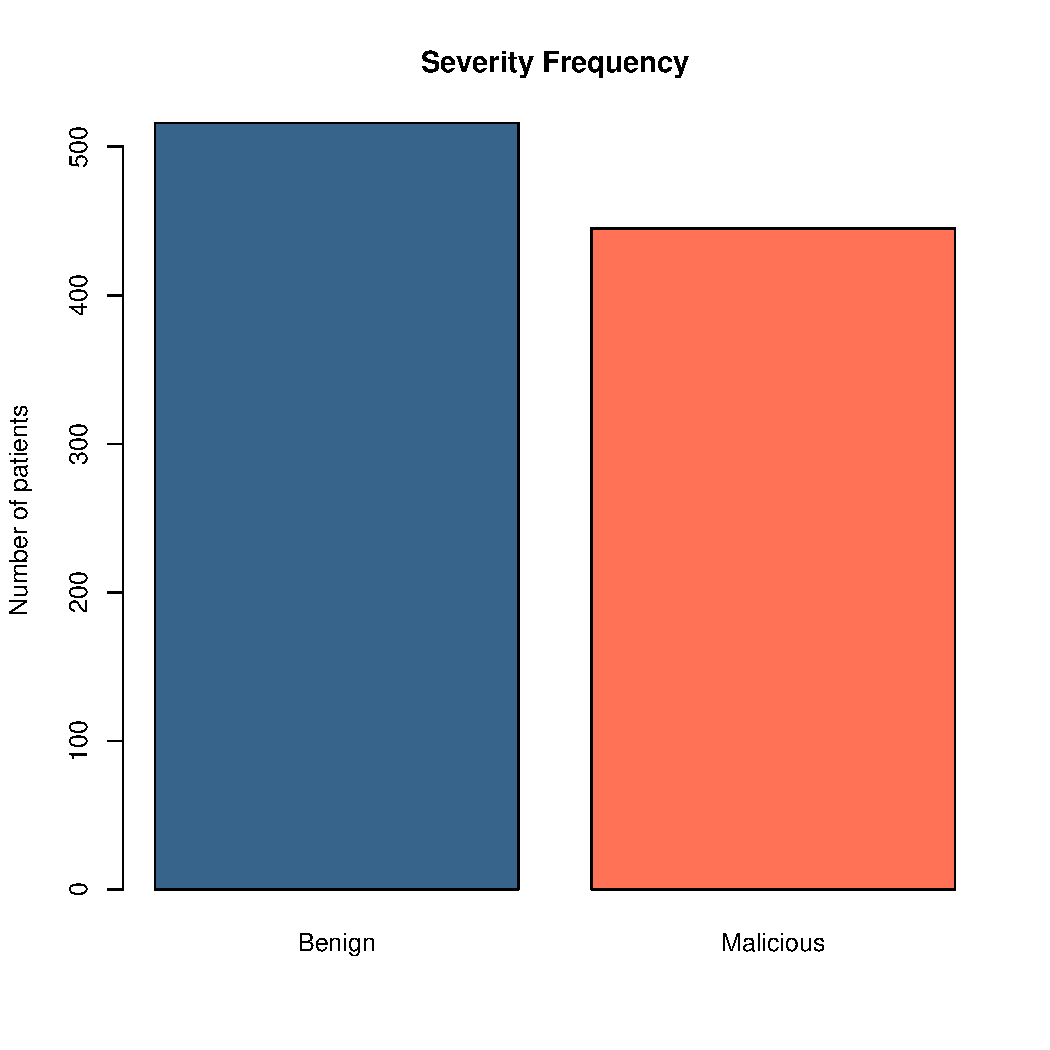
\includegraphics[width=.5\linewidth]{figure/unnamed-chunk-5-1} 

\end{knitrout}
\caption {Class distribution of the severity}
\label{fig1}
}
\end {figure}

\clearpage

\subsubsection{Dataset Summary}\label{summary}

The summary displays a briefing of every column, showing statistical iformation about the data in every entry. The summary can either be numerical (Which shows information such as the maximum and minimum values, median and quartiles) or categorical, which shows the frequency of each one of the categorical values.\\
In this dataset, only the Patient's age is numerical. The rest of the attributes only show the frequency.\\

% Age
{\large Age Summary}\\
The patient Age attribute is a numerical attribute, so the summary shows the minimum, first quartile, median, mean, third quartile and maximum values of the data
\begin{knitrout}
\definecolor{shadecolor}{rgb}{0.969, 0.969, 0.969}\color{fgcolor}\begin{kframe}
\begin{alltt}
\hlcom{# Age    Summary}
\hlkwd{summary}\hlstd{(df}\hlopt{$}\hlstd{Age)}
\end{alltt}
\end{kframe}
\end{knitrout}
\begin{table}[H]
\centering
\begin{tabular}{ c c c c c c c }
Min   & 1st Qu  & Median  & Mean  & 3rd Qu  & Max   & Missing \\
\hline
18.00 & 45.00   & 57.00   & 55.49 & 66.00   & 96.00 & 5
\end{tabular}
\end{table}

\begin{figure}[H]
{\centering
\begin{knitrout}
\definecolor{shadecolor}{rgb}{0.969, 0.969, 0.969}\color{fgcolor}\begin{kframe}
\begin{alltt}
\hlstd{Age} \hlkwb{<-} \hlstd{df}\hlopt{$}\hlstd{Age}
\hlkwd{hist}\hlstd{(}
  \hlstd{Age,}
  \hlkwc{xlab}\hlstd{=}\hlstr{"Patient Age"}\hlstd{,}
  \hlkwc{col}\hlstd{=}\hlstr{"turquoise3"}\hlstd{,}
\hlstd{)}
\end{alltt}
\end{kframe}
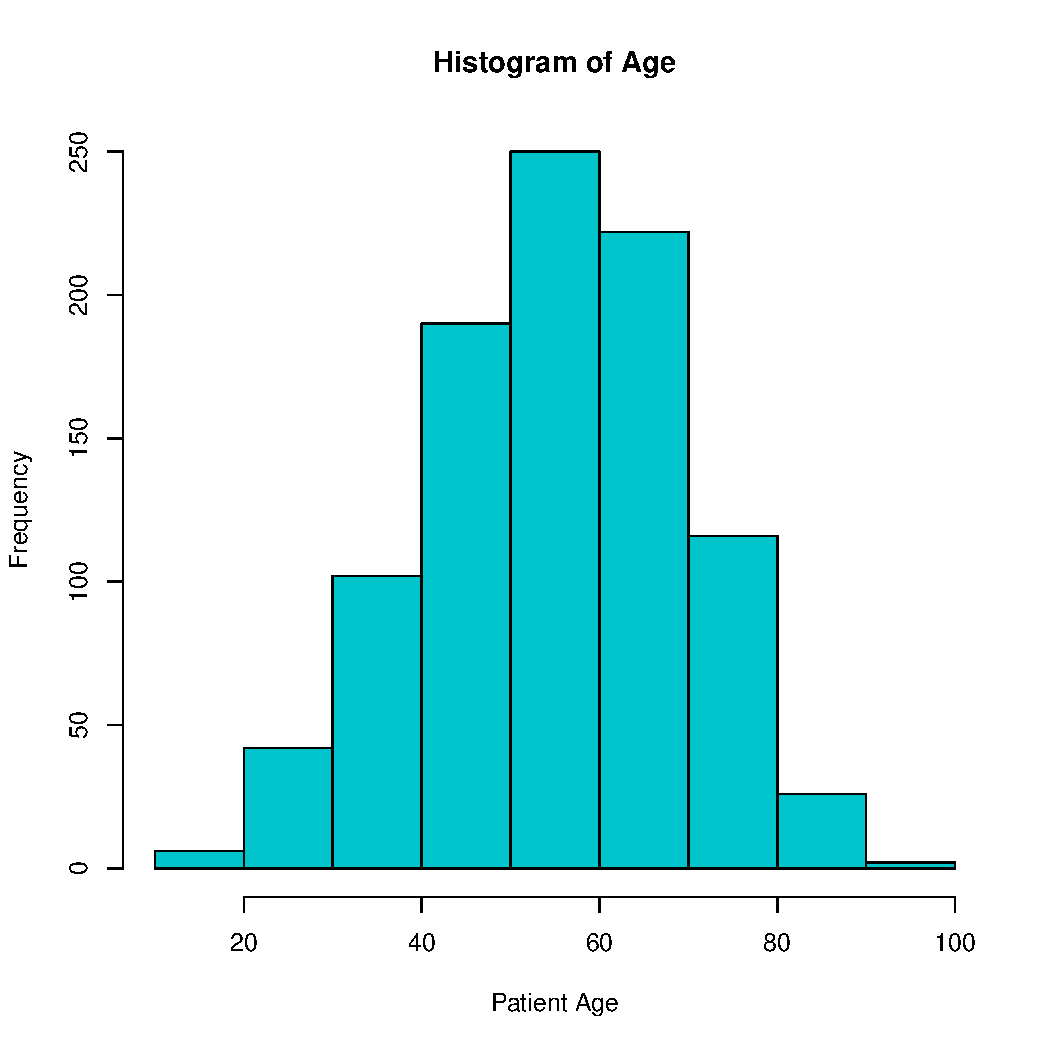
\includegraphics[width=.5\linewidth]{figure/unnamed-chunk-7-1} 

\end{knitrout}
\caption {Histogram of the Patients' Age}
\label{fig2}
}
\end {figure}

% Shape
{\large Shape Summary}\\
The mass Shape attribute is a categorical attribute, so the summary shows the value frequency
\begin{knitrout}
\definecolor{shadecolor}{rgb}{0.969, 0.969, 0.969}\color{fgcolor}\begin{kframe}
\begin{alltt}
\hlcom{# Shape Summary}
\hlkwd{summary}\hlstd{(df}\hlopt{$}\hlstd{Shape)}
\end{alltt}
\end{kframe}
\end{knitrout}
\begin{table}[H]
\centering
\begin{tabular}{ c c c c c }
Round & Oval & Lobular & Irregular & Missing \\
\hline
224   & 211  & 95      & 400       & 31
\end{tabular}
\end{table}

% Margin
{\large Margin Summary}\\
The mass Margin attribute is a categorical attribute, so the summary shows the value frequency
\begin{knitrout}
\definecolor{shadecolor}{rgb}{0.969, 0.969, 0.969}\color{fgcolor}\begin{kframe}
\begin{alltt}
\hlcom{# Margin Summary}
\hlkwd{summary}\hlstd{(df}\hlopt{$}\hlstd{Margin)}
\end{alltt}
\end{kframe}
\end{knitrout}
\begin{table}[H]
\centering
\begin{tabular}{ c c c c c c }
Circumscribed & Microlobulated & Obscured & Ill-defined & Spiculated & Missing \\
\hline
357           & 24             & 116      & 280         & 136        & 48  
\end{tabular}
\end{table}

% Density
{\large Density Summary}\\
The mass Density attribute is a categorical attribute, so the summary shows the value frequency
\begin{knitrout}
\definecolor{shadecolor}{rgb}{0.969, 0.969, 0.969}\color{fgcolor}\begin{kframe}
\begin{alltt}
\hlcom{# Density Summary}
\hlkwd{summary}\hlstd{(df}\hlopt{$}\hlstd{Density)}
\end{alltt}
\end{kframe}
\end{knitrout}
\begin{table}[H]
\centering
\begin{tabular}{ c c c c c }
High  & Iso  & Low  & Fat-Containing & Missing \\
\hline
16    & 59   & 798  & 12             & 76
\end{tabular}
\end{table}

\clearpage

\subsubsection{Attribute Correlation}\label{correlation}
Correlation measures the relationship between two measurements. This dataset only contains one numerical attribute, so there's no chance to create a numerical correlation between the different values. However, a relationship can be established between the age of the patient and the severity of the mammographic mass.This relation is known, but the other attributes also contribute to it.

\begin{figure}[H]
{\centering
\begin{knitrout}
\definecolor{shadecolor}{rgb}{0.969, 0.969, 0.969}\color{fgcolor}\begin{kframe}
\begin{alltt}
\hlcom{# Finding how attributes compare to goal}
\hlkwd{plot}\hlstd{(}
  \hlkwc{data} \hlstd{= df,}
  \hlstd{Age}\hlopt{~}\hlstd{Severity,}
  \hlkwc{col} \hlstd{=} \hlkwd{c}\hlstd{(}\hlstr{'steelblue4'}\hlstd{,}\hlstr{'coral1'}\hlstd{),}
  \hlkwc{names.arg}\hlstd{=}\hlkwd{c}\hlstd{(}\hlstr{"Benign"}\hlstd{,}\hlstr{"Malicious"}\hlstd{)}

\hlstd{)}
\end{alltt}
\end{kframe}
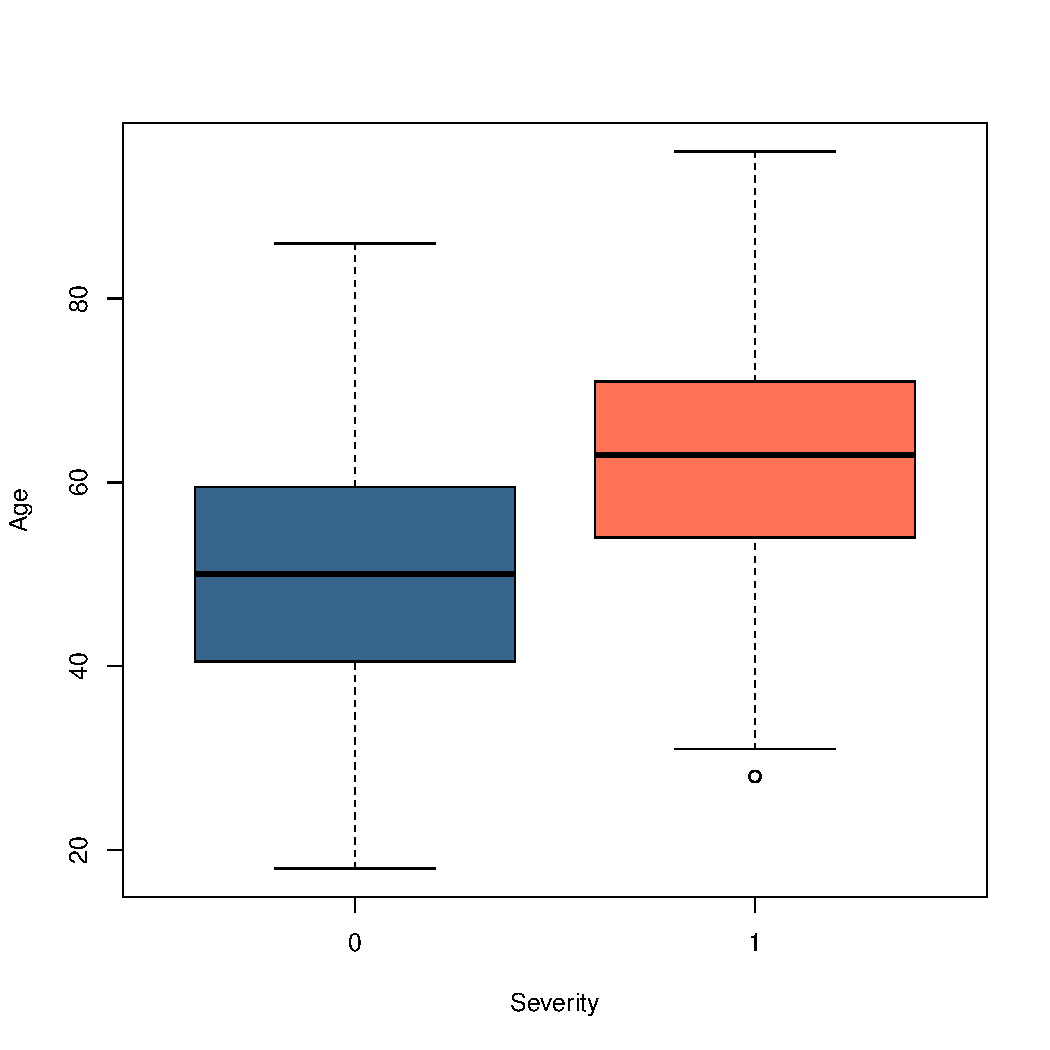
\includegraphics[width=.75\linewidth]{figure/unnamed-chunk-11-1} 

\end{knitrout}
\caption {Correlation between the Age and the severity of the Mammographic mass}
\label{fig3}
}
\end {figure}

\clearpage

In the following page, correlations 3 Age and different Mammographic attributes can be found [~\ref{fig4}], [~\ref{fig5}], [~\ref{fig6}]. As mentioned, there is a relation between the age and the type of mass, but it's not enough to reach a conclusion.

\begin{figure}[H]
{\centering
\begin{knitrout}
\definecolor{shadecolor}{rgb}{0.969, 0.969, 0.969}\color{fgcolor}\begin{kframe}
\begin{alltt}
\hlkwd{library}\hlstd{(datasets)}
\hlstd{data} \hlkwb{<-} \hlkwd{transform}\hlstd{(df, Shape)}
\hlkwd{boxplot}\hlstd{(Age}\hlopt{~}\hlstd{Shape, data,} \hlkwc{xlab}\hlstd{=}\hlstr{"Shape"}\hlstd{,} \hlkwc{ylab}\hlstd{=}\hlstr{"Age"}\hlstd{)}
\end{alltt}
\end{kframe}
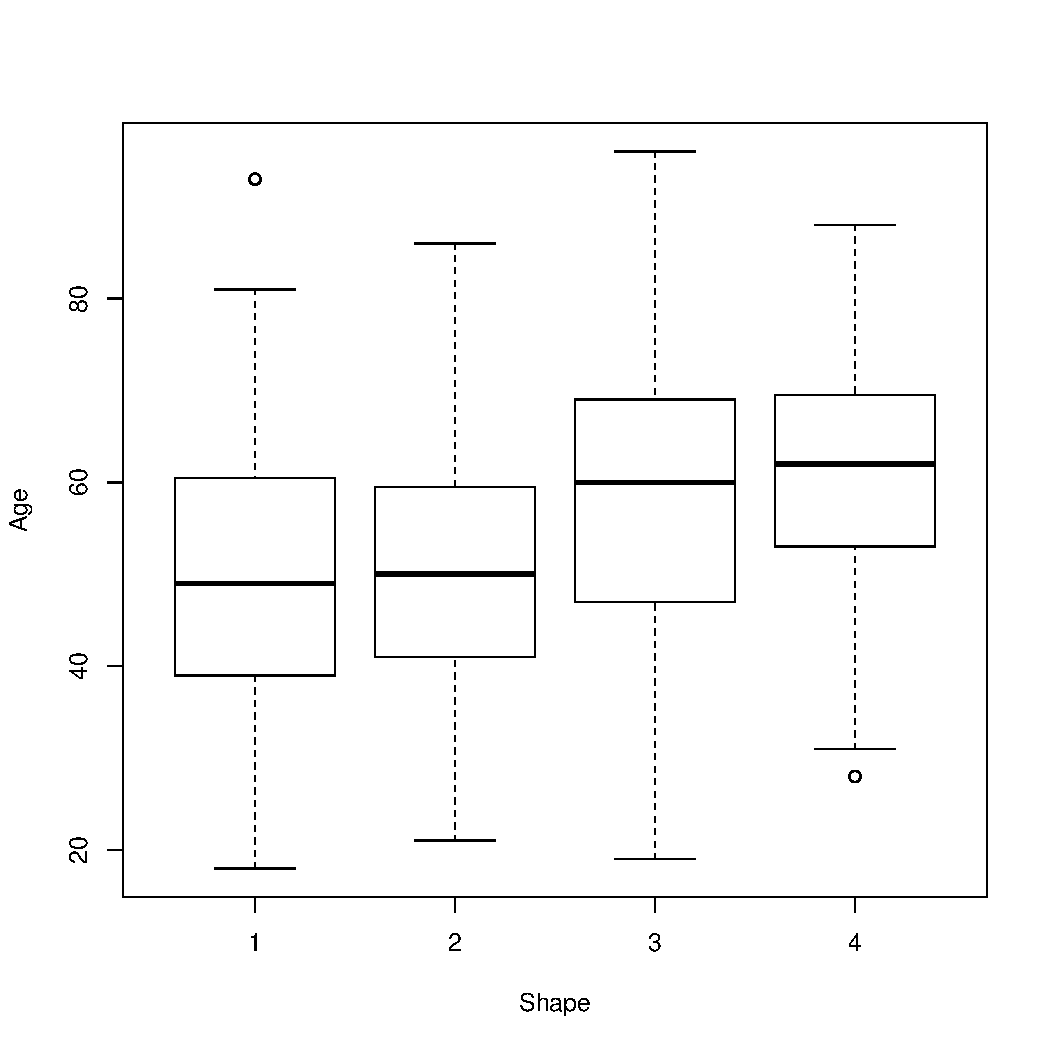
\includegraphics[width=.5\linewidth]{figure/unnamed-chunk-12-1} 

\end{knitrout}
\caption {Relation between Age and Mass Shape (Round, Oval, Lobular, Irregular)}
\label{fig4}
}
\end {figure}

\begin{figure}[H]
{\centering
\begin{knitrout}
\definecolor{shadecolor}{rgb}{0.969, 0.969, 0.969}\color{fgcolor}\begin{kframe}
\begin{alltt}
\hlstd{data} \hlkwb{<-} \hlkwd{transform}\hlstd{(df, Margin)}
\hlkwd{boxplot}\hlstd{(Age}\hlopt{~}\hlstd{Margin, data,}\hlkwc{xlab}\hlstd{=}\hlstr{"Margin"}\hlstd{,}\hlkwc{ylab}\hlstd{=}\hlstr{"Age"}\hlstd{)}
\end{alltt}
\end{kframe}
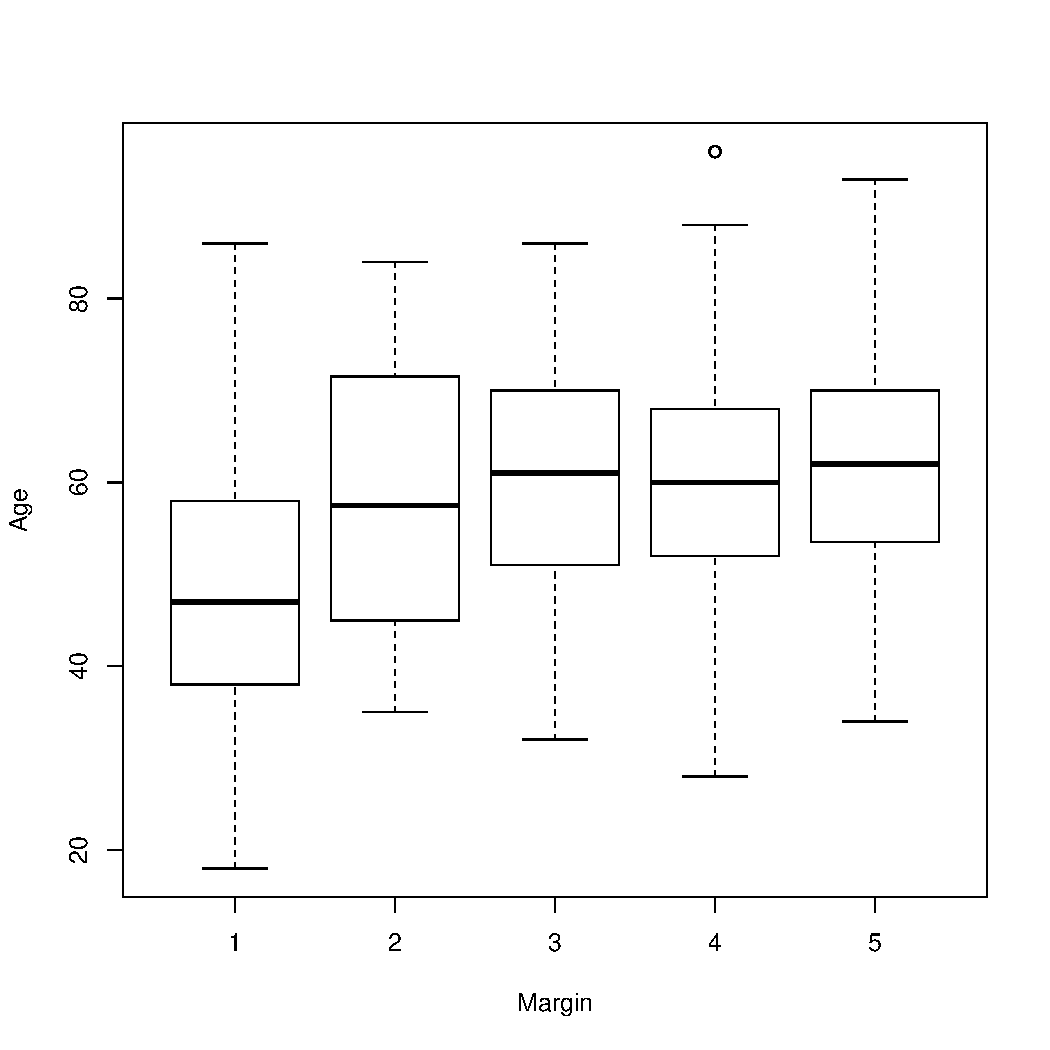
\includegraphics[width=.5\linewidth]{figure/unnamed-chunk-13-1} 

\end{knitrout}
\caption {Relation between Age and Mass Margin (Circumscribed, Microlobulated, Obscured, Ill-defined, Spiculated)}
\label{fig5}
}
\end {figure}

\begin{figure}[H]
{\centering
\begin{knitrout}
\definecolor{shadecolor}{rgb}{0.969, 0.969, 0.969}\color{fgcolor}\begin{kframe}
\begin{alltt}
\hlstd{data} \hlkwb{<-} \hlkwd{transform}\hlstd{(df, Density)}
\hlkwd{boxplot}\hlstd{(Age}\hlopt{~}\hlstd{Density, data,}\hlkwc{xlab}\hlstd{=}\hlstr{"Density"}\hlstd{,}\hlkwc{ylab}\hlstd{=}\hlstr{"Age"}\hlstd{)}
\end{alltt}
\end{kframe}
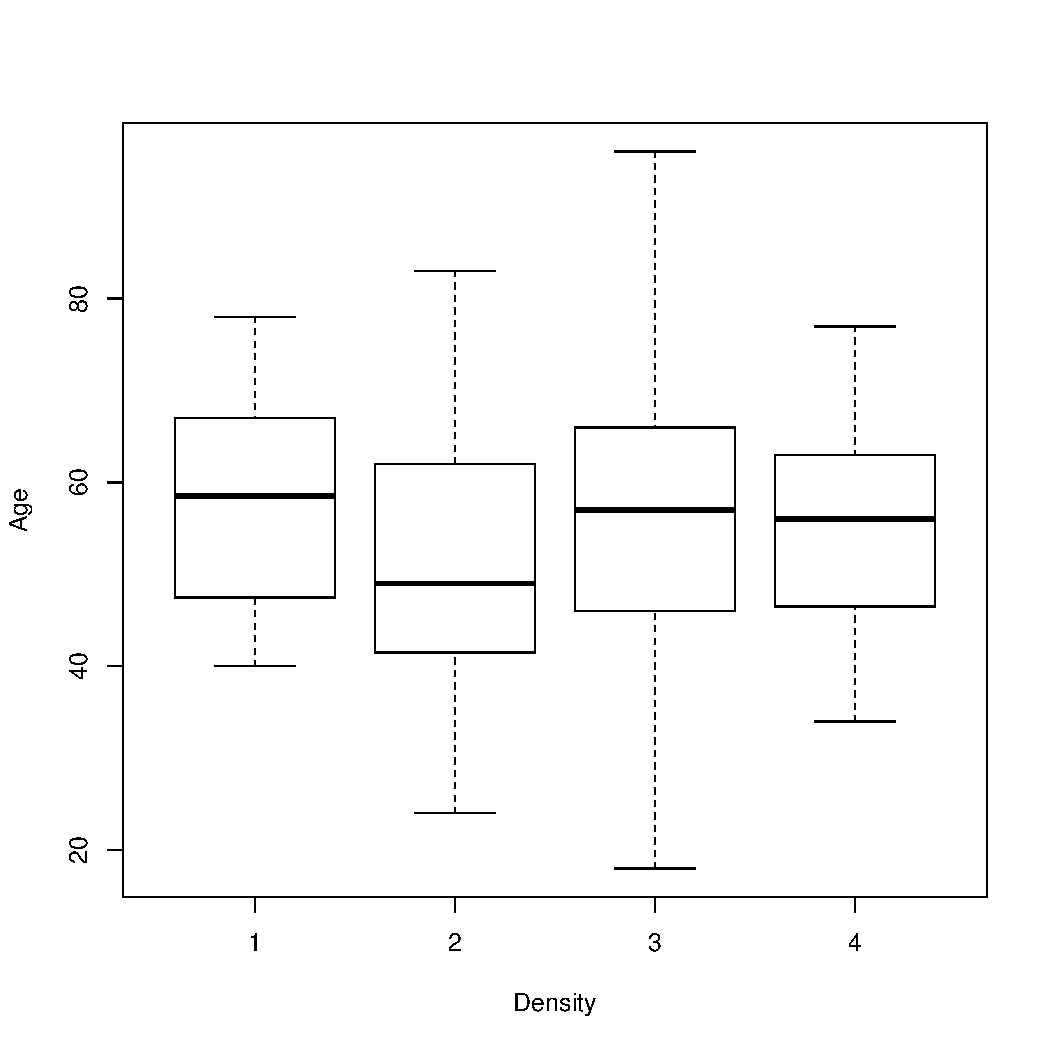
\includegraphics[width=.35\linewidth]{figure/unnamed-chunk-14-1} 

\end{knitrout}
\caption {Relation between Age and the Mass Density (High, Iso, Low, Fat-containing)}
\label{fig6}
}
\end {figure}
  
\clearpage

% Data Pre-processing
\section{Data Pre-processing}\label{preprocess}
In order to analyze the data, the attributes must first be adequated for study. This is known as pre-processing

% Irrelevant Columns
\subsection{Irrelevant Columns}\label{irrelevant_columns}
Before going any further, it has been previously mentioned that the Assessment column is a non-predictive attribute, since it measures the effectiveness of CAD Systems. Therefore, the column is not relevant for data mining, and it should be dropped.

\begin{knitrout}
\definecolor{shadecolor}{rgb}{0.969, 0.969, 0.969}\color{fgcolor}\begin{kframe}
\begin{alltt}
\hlcom{# Backing up the data frame}
\hlstd{df_full} \hlkwb{<-} \hlstd{df}

\hlcom{# Dropping the irrelevant column}
\hlstd{df}\hlopt{$}\hlstd{Assessment} \hlkwb{<-} \hlkwa{NULL}

\hlcom{# Showing the data frame columns without the dropped one}
\hlkwd{names}\hlstd{(df)}
\end{alltt}
\begin{verbatim}
## [1] "Age"      "Shape"    "Margin"   "Density"  "Severity"
\end{verbatim}
\end{kframe}
\end{knitrout}

% Missing Values
\subsection{Missing Values}\label{missing_values}
One of the main issues with the dataset is the number of missing values. When taking a look at the raw data, it can be appreciated that the way missing values were handled was by writing a question mark "?" in place of the value.\\
The data frame will need to have those missing values recognized, so when parsing the file as a data frame, missing values must be specified

\begin{knitrout}
\definecolor{shadecolor}{rgb}{0.969, 0.969, 0.969}\color{fgcolor}\begin{kframe}
\begin{alltt}
\hlcom{# Importing the data}
\hlstd{dataFrame} \hlkwb{<-} \hlkwd{read.table}\hlstd{(}\hlstr{'data/mammographic_masses.data'}\hlstd{,}
                        \hlkwc{header}\hlstd{=}\hlnum{FALSE}\hlstd{,} \hlkwc{sep}\hlstd{=}\hlstr{","}\hlstd{,} \hlkwc{na.strings}\hlstd{=}\hlstr{"?"}\hlstd{)}

\hlcom{# Showing some rows}
\hlstd{df[}\hlnum{1}\hlopt{:}\hlnum{5}\hlstd{,]}
\end{alltt}
\begin{verbatim}
##   Age Shape Margin Density Severity
## 1  67     3      5       3        1
## 2  43     1      1    <NA>        1
## 3  58     4      5       3        1
## 4  28     1      1       3        0
## 5  74     1      5    <NA>        1
\end{verbatim}
\end{kframe}
\end{knitrout}
\clearpage
Now that missing values have been identified, it is necessary to know which values are missing:

\begin{knitrout}
\definecolor{shadecolor}{rgb}{0.969, 0.969, 0.969}\color{fgcolor}\begin{kframe}
\begin{alltt}
\hlkwd{sum}\hlstd{(}\hlkwd{is.na}\hlstd{(df))}
\end{alltt}
\begin{verbatim}
## [1] 160
\end{verbatim}
\begin{alltt}
\hlkwd{sum}\hlstd{(}\hlkwd{is.na}\hlstd{(df}\hlopt{$}\hlstd{Age))}
\end{alltt}
\begin{verbatim}
## [1] 5
\end{verbatim}
\begin{alltt}
\hlkwd{sum}\hlstd{(}\hlkwd{is.na}\hlstd{(df}\hlopt{$}\hlstd{Shape))}
\end{alltt}
\begin{verbatim}
## [1] 31
\end{verbatim}
\begin{alltt}
\hlkwd{sum}\hlstd{(}\hlkwd{is.na}\hlstd{(df}\hlopt{$}\hlstd{Margin))}
\end{alltt}
\begin{verbatim}
## [1] 48
\end{verbatim}
\begin{alltt}
\hlkwd{sum}\hlstd{(}\hlkwd{is.na}\hlstd{(df}\hlopt{$}\hlstd{Density))}
\end{alltt}
\begin{verbatim}
## [1] 76
\end{verbatim}
\begin{alltt}
\hlkwd{sum}\hlstd{(}\hlkwd{is.na}\hlstd{(df}\hlopt{$}\hlstd{Severity))}
\end{alltt}
\begin{verbatim}
## [1] 0
\end{verbatim}
\end{kframe}
\end{knitrout}

\begin{table}[H]
\begin{tabular}{ c c c c c c }
Age & Shape & Margin & Density & Severity & Total \\
\hline
5   & 31    & 48     & 76      & 48       & 162  
\end{tabular}
\end{table}

\clearpage

\subsubsection{Filling missing values}\label{filling_gaps}
With numerical values, a way to deal with missing values is by replacing the blank attribute with the mean of such attribute.
Since the age is the only numerical attribute, we can only use this method here.
\begin{knitrout}
\definecolor{shadecolor}{rgb}{0.969, 0.969, 0.969}\color{fgcolor}\begin{kframe}
\begin{alltt}
\hlcom{# Defining the function}
\hlstd{fillMissings} \hlkwb{<-} \hlkwa{function}\hlstd{(}\hlkwc{x}\hlstd{) \{}
  \hlkwd{replace}\hlstd{(}
    \hlstd{x,}
    \hlkwd{is.na}\hlstd{(x),}
    \hlkwd{mean}\hlstd{(x[}\hlopt{!}\hlkwd{is.na}\hlstd{(x)]))}
\hlstd{\}}

\hlcom{# Applying the function to the Age column}
\hlstd{df}\hlopt{$}\hlstd{Age} \hlkwb{<-} \hlkwd{fillMissings}\hlstd{(df}\hlopt{$}\hlstd{Age)}

\hlcom{# Verifying the number of missing values on the age column}
\hlkwd{sum}\hlstd{(}\hlkwd{is.na}\hlstd{(df}\hlopt{$}\hlstd{Age))}
\end{alltt}
\begin{verbatim}
## [1] 0
\end{verbatim}
\end{kframe}
\end{knitrout}

\subsubsection{Deleting rows}\label{deleting_rows}
Since we cannot fill the missing values, due to the categorical nature of the attributes, we have no other option but to drop the rows that contain them.

\begin{knitrout}
\definecolor{shadecolor}{rgb}{0.969, 0.969, 0.969}\color{fgcolor}\begin{kframe}
\begin{alltt}
\hlcom{# Deleting rows with misssing factor attributes}
\hlstd{df} \hlkwb{<-} \hlstd{df[}\hlopt{!}\hlkwd{is.na}\hlstd{(df}\hlopt{$}\hlstd{Shape),]}
\hlstd{df} \hlkwb{<-} \hlstd{df[}\hlopt{!}\hlkwd{is.na}\hlstd{(df}\hlopt{$}\hlstd{Margin),]}
\hlstd{df} \hlkwb{<-} \hlstd{df[}\hlopt{!}\hlkwd{is.na}\hlstd{(df}\hlopt{$}\hlstd{Density),]}
\end{alltt}
\end{kframe}
\end{knitrout}

We can now observe that there are no missing values in our data frame

\begin{knitrout}
\definecolor{shadecolor}{rgb}{0.969, 0.969, 0.969}\color{fgcolor}\begin{kframe}
\begin{alltt}
\hlkwd{sum}\hlstd{(}\hlkwd{is.na}\hlstd{(df))}
\end{alltt}
\begin{verbatim}
## [1] 0
\end{verbatim}
\end{kframe}
\end{knitrout}

\clearpage

% Missing Header
\subsection{Missing Header}\label{missing_header}
Another issue with the dataset is the lack of headers. We may know the meaning of every column after reading about the dataset, but we still need a way to identify each one of the columns.

\begin{knitrout}
\definecolor{shadecolor}{rgb}{0.969, 0.969, 0.969}\color{fgcolor}\begin{kframe}
\begin{alltt}
\hlcom{# Showing the data frame header}
\hlkwd{names}\hlstd{(dataFrame)}
\end{alltt}
\begin{verbatim}
## [1] "V1" "V2" "V3" "V4" "V5" "V6"
\end{verbatim}
\begin{alltt}
\hlcom{# Changing the column names}
\hlkwd{names}\hlstd{(dataFrame)} \hlkwb{<-} \hlkwd{c}\hlstd{(}\hlstr{"Assessment"}\hlstd{,}\hlstr{"Age"}\hlstd{,}\hlstr{"Shape"}\hlstd{,}\hlstr{"Margin"}\hlstd{,}\hlstr{"Density"}\hlstd{,} \hlstr{"Severity"}\hlstd{)}

\hlcom{# Showing the column names}
\hlkwd{names}\hlstd{(dataFrame)}
\end{alltt}
\begin{verbatim}
## [1] "Assessment" "Age"        "Shape"      "Margin"     "Density"   
## [6] "Severity"
\end{verbatim}
\end{kframe}
\end{knitrout}

\subsection{Categorical Values}\label{categorical_values}
As previously mentioned, most of the values are categorical, rather than numerical. This means that it can't just be measured as a number, but as propertie of the entries. After dropping unnecessary columns, the categorical attributes are the following:

\begin{enumerate}
\item \textbf{Shape}: Shape of the mammographic mass. (Nominal)
\item \textbf{Margin}: Margin of the mammographic mass. (Nominal)
\item \textbf{Density}: Density of the mammographic mass. (Ordinal)
\item \textbf{Severity}: Severity of the mammographic mass. (Binominal)
\end{enumerate}

Fortunately enough, the categorical attributes already come as numerical values. If this was not the case and they were represented as, for instance, strings, such strings would need to be converted into numerical values.\\
Now, the attributes will be converted into categorical values.

\begin{knitrout}
\definecolor{shadecolor}{rgb}{0.969, 0.969, 0.969}\color{fgcolor}\begin{kframe}
\begin{alltt}
\hlcom{# Turning the attributes into categofical}
\hlstd{df}\hlopt{$}\hlstd{Shape}      \hlkwb{<-} \hlkwd{factor}\hlstd{(df}\hlopt{$}\hlstd{Shape)}
\hlstd{df}\hlopt{$}\hlstd{Margin}     \hlkwb{<-} \hlkwd{factor}\hlstd{(df}\hlopt{$}\hlstd{Margin)}
\hlstd{df}\hlopt{$}\hlstd{Density}    \hlkwb{<-} \hlkwd{factor}\hlstd{(df}\hlopt{$}\hlstd{Density,} \hlkwc{order}\hlstd{=}\hlnum{TRUE}\hlstd{,} \hlkwc{levels}\hlstd{=}\hlkwd{c}\hlstd{(}\hlstr{"1"}\hlstd{,}\hlstr{"2"}\hlstd{,}\hlstr{"3"}\hlstd{,}\hlstr{"4"}\hlstd{))}
\hlstd{df}\hlopt{$}\hlstd{Severity}   \hlkwb{<-} \hlkwd{factor}\hlstd{(df}\hlopt{$}\hlstd{Severity)}

\hlcom{# Checking whether the fields are factors}
\hlkwd{is.factor}\hlstd{(df}\hlopt{$}\hlstd{Age)}
\end{alltt}
\begin{verbatim}
## [1] FALSE
\end{verbatim}
\begin{alltt}
\hlkwd{is.factor}\hlstd{(df}\hlopt{$}\hlstd{Shape)}
\end{alltt}
\begin{verbatim}
## [1] TRUE
\end{verbatim}
\begin{alltt}
\hlkwd{is.factor}\hlstd{(df}\hlopt{$}\hlstd{Margin)}
\end{alltt}
\begin{verbatim}
## [1] TRUE
\end{verbatim}
\begin{alltt}
\hlkwd{is.factor}\hlstd{(df}\hlopt{$}\hlstd{Density)}
\end{alltt}
\begin{verbatim}
## [1] TRUE
\end{verbatim}
\begin{alltt}
\hlkwd{is.factor}\hlstd{(df}\hlopt{$}\hlstd{Severity)}
\end{alltt}
\begin{verbatim}
## [1] TRUE
\end{verbatim}
\end{kframe}
\end{knitrout}

\subsection{Data Normalization}\label{data_normalization}
Since there are no noticeable irregularities in the dataset, such as outliers or skewed values, there is no need to normalize the dataset.

\clearpage

% Modelling Section

\section{Modelling}\label{modelling}
Now that the dataset has been explored and there is a better idea of what needs to be predicted, we can start building and testing models.

\begin{knitrout}
\definecolor{shadecolor}{rgb}{0.969, 0.969, 0.969}\color{fgcolor}\begin{kframe}
\begin{alltt}
\hlcom{# Downloading necessary libraries}
\hlkwd{library}\hlstd{(ISLR)}
\hlkwd{library}\hlstd{(dplyr)}
\hlkwd{library}\hlstd{(ROCR)}
\end{alltt}
\end{kframe}
\end{knitrout}

\subsection{Creating Subsets}\label{subsets}
Before creating predictive models, the dataset will be split into a training and a testing set, in order to avoid future problems with overfitting or underfitting.

\begin{knitrout}
\definecolor{shadecolor}{rgb}{0.969, 0.969, 0.969}\color{fgcolor}\begin{kframe}
\begin{alltt}
\hlcom{# Dividing a dataset into train and test}
\hlstd{createSubsets} \hlkwb{<-} \hlkwa{function} \hlstd{(}\hlkwc{dataset}\hlstd{,} \hlkwc{percentage}\hlstd{) \{}

  \hlcom{# Getting the training dataset}
  \hlstd{train}\hlkwb{<-}\hlkwd{sample_frac}\hlstd{( dataset , percentage)}
  \hlstd{sid}\hlkwb{<-}\hlkwd{as.numeric}\hlstd{(}\hlkwd{rownames}\hlstd{(train))}

  \hlcom{# Getting the test dataset}
  \hlstd{validation} \hlkwb{<-} \hlstd{dataset[}\hlopt{-}\hlstd{sid,]}

  \hlcom{# Returning the 2 subsets}
  \hlkwd{return}\hlstd{(}\hlkwd{list}\hlstd{(}\hlstr{"train"}\hlstd{=train,} \hlstr{"validation"}\hlstd{=validation))}
\hlstd{\}}

\hlstd{subset} \hlkwb{<-} \hlkwd{createSubsets}\hlstd{(df,} \hlnum{0.7}\hlstd{)}

\hlstd{train} \hlkwb{<-} \hlstd{subset}\hlopt{$}\hlstd{train}
\hlkwd{nrow}\hlstd{(train)}
\end{alltt}
\begin{verbatim}
## [1] 585
\end{verbatim}
\begin{alltt}
\hlstd{validation} \hlkwb{<-} \hlstd{subset}\hlopt{$}\hlstd{validation}
\hlkwd{nrow}\hlstd{(validation)}
\end{alltt}
\begin{verbatim}
## [1] 251
\end{verbatim}
\begin{alltt}
\hlkwa{if} \hlstd{(} \hlkwd{nrow}\hlstd{(train)} \hlopt{+} \hlkwd{nrow}\hlstd{(validation)} \hlopt{==} \hlkwd{nrow}\hlstd{(df) )\{}
  \hlkwd{print}\hlstd{(}\hlstr{"The dataset has been split properly"}\hlstd{)}
\hlstd{\}} \hlkwa{else} \hlstd{\{}
  \hlkwd{print}\hlstd{(}\hlstr{"The split of the dataset was not correct"}\hlstd{)}
\hlstd{\}}
\end{alltt}
\begin{verbatim}
## [1] "The dataset has been split properly"
\end{verbatim}
\end{kframe}
\end{knitrout}

\clearpage

\subsection{Implementing a Model}\label{model}
Now that the dataset has been split, the training subset can be used to start designing the model. For this case, Logistic Regression will be used. Logistic regression is used to model the probability that an ‘event’ will occur. In other words, the dependent variable, now p(X), assumes a value between 0 and 1. This is suitable for the current dataset, since what we are trying to predict is whether a mammographic mass can be benign of malicious (0 or 1).

\begin{knitrout}
\definecolor{shadecolor}{rgb}{0.969, 0.969, 0.969}\color{fgcolor}\begin{kframe}
\begin{alltt}
\hlcom{# Implementing the Logistic Regression model}

\hlstd{createRegressionModel} \hlkwb{<-} \hlkwa{function} \hlstd{(}\hlkwc{dataset}\hlstd{) \{}
  \hlkwd{return}\hlstd{(} \hlkwd{glm}\hlstd{(}
    \hlstd{Severity} \hlopt{~} \hlstd{Age}\hlopt{+}\hlstd{Shape}\hlopt{+}\hlstd{Margin}\hlopt{+}\hlstd{Density,} \hlcom{# Severity against parameters}
    \hlkwc{data}\hlstd{=dataset,}                        \hlcom{# Using training data}
    \hlkwc{family}\hlstd{=binomial}                      \hlcom{# Goal is a binomial value}
  \hlstd{))}
\hlstd{\}}

\hlcom{# Spitting the summary of the model}
\hlstd{regressionModel} \hlkwb{<-} \hlkwd{createRegressionModel}\hlstd{(train)}
\hlkwd{summary}\hlstd{(regressionModel)}
\end{alltt}
\begin{verbatim}
## 
## Call:
## glm(formula = Severity ~ Age + Shape + Margin + Density, family = binomial, 
##     data = dataset)
## 
## Deviance Residuals: 
##     Min       1Q   Median       3Q      Max  
## -2.6264  -0.5683   0.2396   0.6393   2.5580  
## 
## Coefficients:
##              Estimate Std. Error z value Pr(>|z|)    
## (Intercept) -4.966846   0.680924  -7.294 3.00e-13 ***
## Age          0.059649   0.009496   6.281 3.36e-10 ***
## Shape2      -0.173999   0.373242  -0.466 0.641086    
## Shape3       0.517236   0.454117   1.139 0.254706    
## Shape4       1.498870   0.390863   3.835 0.000126 ***
## Margin2      1.614717   0.692694   2.331 0.019750 *  
## Margin3      1.314278   0.415741   3.161 0.001571 ** 
## Margin4      1.433762   0.355324   4.035 5.46e-05 ***
## Margin5      1.994361   0.441820   4.514 6.36e-06 ***
## Density.L   -0.597975   0.931918  -0.642 0.521094    
## Density.Q    0.349678   0.720520   0.485 0.627455    
## Density.C   -0.280886   0.427679  -0.657 0.511329    
## ---
## Signif. codes:  0 '***' 0.001 '**' 0.01 '*' 0.05 '.' 0.1 ' ' 1
## 
## (Dispersion parameter for binomial family taken to be 1)
## 
##     Null deviance: 810.94  on 584  degrees of freedom
## Residual deviance: 505.86  on 573  degrees of freedom
## AIC: 529.86
## 
## Number of Fisher Scoring iterations: 5
\end{verbatim}
\end{kframe}
\end{knitrout}

\subsection{Model Evaluation}\label{evaluation}
After applying certain model to a dataset it is necessary to evaluate its performance. In order to dot that, a confusion matrix will be used, in which the prediction column that was produced during the model needs to be tested against the actual class values that already existed on the dataset. This will produce the following possible results:
\begin{itemize}
  \item \textbf{True Positive (TP)}: correctly classified as the class of interest
  \item \textbf{True Negative(TN)}: Correctly classified as not the class of interest
  \item \textbf{False Positive(FP)}: Incorrectly classified as the class of interest
  \item \textbf{False Negative(FN)}: Incorrectly classified as not the class of interest
\end{itemize}

In order to perform a thorough analysis of the performance, it is advisable to predict the severity of the mammographic masses against the validation subset. In order to do that, a prediction is created by using the model and the testing dataset, with which the accuracy can be calculated.

\begin{knitrout}
\definecolor{shadecolor}{rgb}{0.969, 0.969, 0.969}\color{fgcolor}\begin{kframe}
\begin{alltt}
\hlcom{# Get the accuracy of the model}
\hlstd{getModelAccuracy} \hlkwb{<-} \hlkwa{function} \hlstd{(}\hlkwc{dataset}\hlstd{,} \hlkwc{model}\hlstd{) \{}
  \hlcom{# Generating a prediction}
  \hlstd{probabilities} \hlkwb{<-} \hlkwd{predict}\hlstd{(}
    \hlstd{model,}                                     \hlcom{# Used model}
    \hlkwc{newdata}\hlstd{=}\hlkwd{subset}\hlstd{(dataset,}\hlkwc{select}\hlstd{=}\hlkwd{c}\hlstd{(}\hlnum{1}\hlstd{,}\hlnum{2}\hlstd{,}\hlnum{3}\hlstd{,}\hlnum{4}\hlstd{)),} \hlcom{# Test dataset}
    \hlkwc{type}\hlstd{=}\hlstr{"response"}                            \hlcom{# Type of prediction}
  \hlstd{)}

  \hlcom{# Store the predictions as 1 or 0}
  \hlstd{predictions} \hlkwb{<-} \hlkwd{ifelse}\hlstd{(probabilities}\hlopt{>}\hlnum{0.5}\hlstd{,} \hlnum{1}\hlstd{,} \hlnum{0}\hlstd{)}

  \hlcom{# Store accuracy}
  \hlstd{accuracy} \hlkwb{=} \hlkwd{mean}\hlstd{(predictions}\hlopt{==}\hlstd{validation}\hlopt{$}\hlstd{Severity)}

  \hlcom{# Return Accuracy}
  \hlkwd{return}\hlstd{(} \hlkwd{list}\hlstd{(}\hlstr{"probabilities"}\hlstd{=probabilities,}
               \hlstr{"predictions"}\hlstd{=predictions,}
               \hlstr{"accuracy"}\hlstd{=accuracy))}
\hlstd{\}}

\hlcom{# Output the accuracy}
\hlstd{accuracyList} \hlkwb{=} \hlkwd{getModelAccuracy}\hlstd{(validation,regressionModel)}
\hlstd{accuracyList}\hlopt{$}\hlstd{accuracy}
\end{alltt}
\begin{verbatim}
## [1] 0.8446215
\end{verbatim}
\end{kframe}
\end{knitrout}

Finally, a ROC curve can be used to measure the performance of a model:
\begin{itemize}
  \item The true positive rate is the sensitivity: the fraction of defaulters that are correctly identified, using a given threshold value.
  \item The false positive rate is 1-specificity: the fraction of non-defaulters that we classify incorrectly as defaulters, using that same threshold value.
\end{itemize}

\begin{figure}[H]
{\centering
\begin{knitrout}
\definecolor{shadecolor}{rgb}{0.969, 0.969, 0.969}\color{fgcolor}\begin{kframe}
\begin{alltt}
\hlcom{# ROC Model}
\hlstd{pr} \hlkwb{<-} \hlkwd{prediction}\hlstd{(accuracyList}\hlopt{$}\hlstd{probabilities, validation}\hlopt{$}\hlstd{Severity)}
\hlstd{prf} \hlkwb{<-} \hlkwd{performance}\hlstd{( pr,} \hlkwc{measure} \hlstd{=} \hlstr{"tpr"}\hlstd{,} \hlkwc{x.measure} \hlstd{=} \hlstr{"fpr"}\hlstd{)}
\hlkwd{plot}\hlstd{(prf,}\hlkwc{frame}\hlstd{=}\hlnum{FALSE}\hlstd{)}
\end{alltt}
\end{kframe}
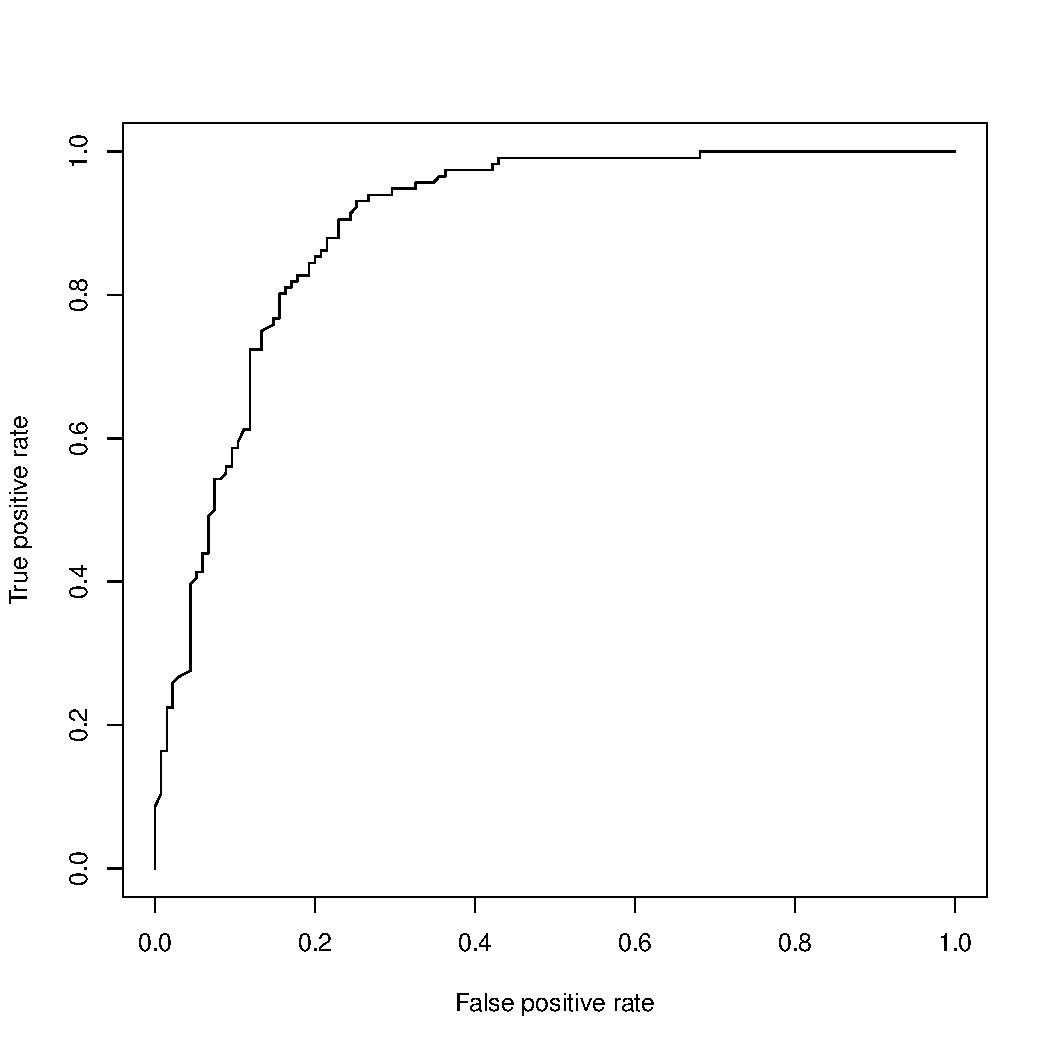
\includegraphics[width=.5\linewidth]{figure/unnamed-chunk-27-1} 

\end{knitrout}
\caption {ROC curve of the regression model}
\label{fig7}
}
\end {figure}

\clearpage

\section{Improving Performance}\label{improving_performance}
Even though the model has achieved a fairly decent performance, it can definitely be improved. Small tweaks in the dataset, model and validation might have a positive impact on the accuracy, which would lead to a more trustworthy prediction of a potential malignant lesion, hence saving lives. I've chosen the following methods to improve my dataset's model:
\begin{itemize}
  \item \textbf{Filling missing values}: By dealing with missing values in a better way, the dataset size may increase, which leads to more accurate models.
  \item \textbf{Cross Validation}: When using training and testing datasets, there must be a tradeoff between maximizing training and validation dataset size, which can lead to inaccurate models. By using different validation methods, the performance of a given model may increase.
  \item \textbf{Different Models}: Using different modelling algorithms may vary the prediction accuracy for any given dataset, so it is a good idea to use more complex models.
\end{itemize}

\begin{knitrout}
\definecolor{shadecolor}{rgb}{0.969, 0.969, 0.969}\color{fgcolor}\begin{kframe}
\begin{alltt}
\hlcom{# Downloading necessary libraries}
\hlkwd{library}\hlstd{(caret)}
\hlkwd{library}\hlstd{(mice)}
\end{alltt}
\end{kframe}
\end{knitrout}

\subsection{Filling Missing Values}\label{filling_missing}
Having a large enough dataset is a very relevant factor when it comes to perfecting a machine learning algorithm. The bigger the training data, the better the adjustments, and the more accurate the system may become. On any given dataset, there may be missing values, and while sometimes there is no way to recreate such missing values and entire rows must be dropped, an effort must be made in order to save as much information as possible.\\
Earlier in this coursework, it was assumed that all missing categorical values were supposed to be deleted, without trying to handle them. However, this was a mistake, and there are sevetral algorithms that deal with missing categorical values \cite{mekala_2019}. In this case, the package of choice has been MICE (Multivariate Imputation via Chained Equations), one of the commonly used package by R users. Creating multiple imputations as compared to a single imputation takes care of uncertainty in missing values. MICE assumes that the missing data are Missing at Random (MAR), which means that the probability that a value is missing depends only on observed value and can be predicted using them. It imputes data on a variable by variable basis by specifying an imputation model per variable.

\begin{knitrout}
\definecolor{shadecolor}{rgb}{0.969, 0.969, 0.969}\color{fgcolor}\begin{kframe}
\begin{alltt}
\hlcom{# Getting our new dataframe ready}
\hlstd{new_df} \hlkwb{<-} \hlstd{df_full}
\hlstd{new_df}\hlopt{$}\hlstd{Assessment} \hlkwb{<-} \hlkwa{NULL}
\hlstd{new_df}\hlopt{$}\hlstd{Age} \hlkwb{<-} \hlkwd{fillMissings}\hlstd{(new_df}\hlopt{$}\hlstd{Age)}

\hlcom{# Using MICE to fill missing categorical values}
\hlstd{new_df} \hlkwb{<-} \hlkwd{mice}\hlstd{(}
  \hlstd{new_df,}           \hlcom{# Using the newDF dataframe}
  \hlkwc{m}\hlstd{=}\hlnum{1}\hlstd{,}              \hlcom{# Generating only 1 dataframe}
  \hlkwc{maxit}\hlstd{=}\hlnum{20}\hlstd{,}         \hlcom{# Number of Iterations}
  \hlkwc{method}\hlstd{=}\hlstr{'polyreg'}\hlstd{,} \hlcom{# Polyreg imputation Method for categorical values}
  \hlkwc{seed}\hlstd{=}\hlnum{666}          \hlcom{# Seed}
\hlstd{)}
\end{alltt}
\begin{verbatim}
## 
##  iter imp variable
##   1   1  Shape  Margin  Density
##   2   1  Shape  Margin  Density
##   3   1  Shape  Margin  Density
##   4   1  Shape  Margin  Density
##   5   1  Shape  Margin  Density
##   6   1  Shape  Margin  Density
##   7   1  Shape  Margin  Density
##   8   1  Shape  Margin  Density
##   9   1  Shape  Margin  Density
##   10   1  Shape  Margin  Density
##   11   1  Shape  Margin  Density
##   12   1  Shape  Margin  Density
##   13   1  Shape  Margin  Density
##   14   1  Shape  Margin  Density
##   15   1  Shape  Margin  Density
##   16   1  Shape  Margin  Density
##   17   1  Shape  Margin  Density
##   18   1  Shape  Margin  Density
##   19   1  Shape  Margin  Density
##   20   1  Shape  Margin  Density
\end{verbatim}
\begin{alltt}
\hlcom{# Choosing the generated dataframe}
\hlstd{new_df} \hlkwb{<-} \hlkwd{complete}\hlstd{(new_df,}\hlnum{1}\hlstd{)}

\hlcom{# Checking the number of missing values}
\hlkwd{sum}\hlstd{(}\hlkwd{is.na}\hlstd{(new_df))}
\end{alltt}
\begin{verbatim}
## [1] 0
\end{verbatim}
\end{kframe}
\end{knitrout}

\clearpage

\subsection{Cross Validation}\label{cross_validation}
As mentioned earlier, dividing datasets into training and a validation subsets is an easy way to train a model, but it can lead to tradeoffs during the different stages of the model creation. There are many ways to validate models, but in this case the best approach is to use Cross Validation method. The k-fold cross validation method involves splitting the dataset into k-subsets. During the training phase each subset is held out while the model is trained on all other subsets. This process is completed until accuracy is determine for each instance in the dataset, and an overall accuracy estimate is provided.

\begin{knitrout}
\definecolor{shadecolor}{rgb}{0.969, 0.969, 0.969}\color{fgcolor}\begin{kframe}
\begin{alltt}
\hlcom{# Create a partition, to reserve a validation subset for later testing}
\hlstd{inTrain} \hlkwb{<-} \hlkwd{createDataPartition}\hlstd{(}
  \hlkwc{y}\hlstd{=new_df}\hlopt{$}\hlstd{Severity,} \hlcom{# Have Severity as the classifying value}
  \hlkwc{p}\hlstd{=}\hlnum{0.7}\hlstd{,}            \hlcom{# Assign 75% of the data to training}
  \hlkwc{list}\hlstd{=}\hlnum{FALSE}
\hlstd{)}

\hlcom{# Generating the training subset}
\hlstd{new_training} \hlkwb{<-} \hlstd{new_df[inTrain,]}
\hlkwd{nrow}\hlstd{(new_training)}
\end{alltt}
\begin{verbatim}
## [1] 674
\end{verbatim}
\begin{alltt}
\hlcom{# Generating the validating subset}
\hlstd{new_validating} \hlkwb{<-} \hlstd{new_df [}\hlopt{-}\hlstd{inTrain,]}
\hlkwd{nrow}\hlstd{(new_validating)}
\end{alltt}
\begin{verbatim}
## [1] 287
\end{verbatim}
\begin{alltt}
\hlcom{# Cross Validation}
\hlstd{train_control}\hlkwb{<-} \hlkwd{trainControl}\hlstd{(}
  \hlkwc{method}\hlstd{=}\hlstr{"cv"}\hlstd{,}\hlcom{# Use the Cross Validation Method}
  \hlkwc{number}\hlstd{=}\hlnum{10}\hlstd{,}  \hlcom{# Divide into 10 subsets#}
\hlstd{)}
\end{alltt}
\end{kframe}
\end{knitrout}

\clearpage

\subsection{Different Models}\label{different_models}
On this particular dataset, having an accurate prediction can drastically influence a patient, since a false negative means that a  mammographic mass could develop into a potentially untreated cancerous condition.\\
The previously used logistic regression algorithm may have given decent results, but it still might be a good idea to test a different model. In this case, the chosen predictive model will be "Random Forest", which consists of a large number of individual decision trees that operate as an ensemble. Each individual tree in the random forest spits out a class prediction and the class with the most votes becomes our model’s prediction \cite{yiu_2019}.

\begin{knitrout}
\definecolor{shadecolor}{rgb}{0.969, 0.969, 0.969}\color{fgcolor}\begin{kframe}
\begin{alltt}
\hlcom{# Random Forest}
\hlstd{randomForestModel}\hlkwb{<-} \hlkwd{train}\hlstd{(}
  \hlstd{Severity}\hlopt{~}\hlstd{.,}                \hlcom{# Severity is the value to predict}
  \hlkwc{data}\hlstd{=new_training,}         \hlcom{# Use the training data}
  \hlkwc{trControl}\hlstd{=train_control,}   \hlcom{# Use Cross Validation}
  \hlkwc{method}\hlstd{=}\hlstr{"ranger"}\hlstd{,}           \hlcom{# Use Random Forest}
  \hlkwc{family}\hlstd{=}\hlkwd{binomial}\hlstd{()}          \hlcom{# The value to predict is binomial}
\hlstd{)}
\end{alltt}


{\ttfamily\noindent\color{warningcolor}{\#\# Warning: model fit failed for Fold01: mtry= 2, min.node.size=1, splitrule=gini Error in ranger::ranger(dependent.variable.name = "{}.outcome"{}, data = x,\ \ : \\\#\#\ \  unused argument (family = binomial())}}

{\ttfamily\noindent\color{warningcolor}{\#\# Warning: model fit failed for Fold01: mtry= 6, min.node.size=1, splitrule=gini Error in ranger::ranger(dependent.variable.name = "{}.outcome"{}, data = x,\ \ : \\\#\#\ \  unused argument (family = binomial())}}

{\ttfamily\noindent\color{warningcolor}{\#\# Warning: model fit failed for Fold01: mtry=11, min.node.size=1, splitrule=gini Error in ranger::ranger(dependent.variable.name = "{}.outcome"{}, data = x,\ \ : \\\#\#\ \  unused argument (family = binomial())}}

{\ttfamily\noindent\color{warningcolor}{\#\# Warning: model fit failed for Fold01: mtry= 2, min.node.size=1, splitrule=extratrees Error in ranger::ranger(dependent.variable.name = "{}.outcome"{}, data = x,\ \ : \\\#\#\ \  unused argument (family = binomial())}}

{\ttfamily\noindent\color{warningcolor}{\#\# Warning: model fit failed for Fold01: mtry= 6, min.node.size=1, splitrule=extratrees Error in ranger::ranger(dependent.variable.name = "{}.outcome"{}, data = x,\ \ : \\\#\#\ \  unused argument (family = binomial())}}

{\ttfamily\noindent\color{warningcolor}{\#\# Warning: model fit failed for Fold01: mtry=11, min.node.size=1, splitrule=extratrees Error in ranger::ranger(dependent.variable.name = "{}.outcome"{}, data = x,\ \ : \\\#\#\ \  unused argument (family = binomial())}}

{\ttfamily\noindent\color{warningcolor}{\#\# Warning: model fit failed for Fold02: mtry= 2, min.node.size=1, splitrule=gini Error in ranger::ranger(dependent.variable.name = "{}.outcome"{}, data = x,\ \ : \\\#\#\ \  unused argument (family = binomial())}}

{\ttfamily\noindent\color{warningcolor}{\#\# Warning: model fit failed for Fold02: mtry= 6, min.node.size=1, splitrule=gini Error in ranger::ranger(dependent.variable.name = "{}.outcome"{}, data = x,\ \ : \\\#\#\ \  unused argument (family = binomial())}}

{\ttfamily\noindent\color{warningcolor}{\#\# Warning: model fit failed for Fold02: mtry=11, min.node.size=1, splitrule=gini Error in ranger::ranger(dependent.variable.name = "{}.outcome"{}, data = x,\ \ : \\\#\#\ \  unused argument (family = binomial())}}

{\ttfamily\noindent\color{warningcolor}{\#\# Warning: model fit failed for Fold02: mtry= 2, min.node.size=1, splitrule=extratrees Error in ranger::ranger(dependent.variable.name = "{}.outcome"{}, data = x,\ \ : \\\#\#\ \  unused argument (family = binomial())}}

{\ttfamily\noindent\color{warningcolor}{\#\# Warning: model fit failed for Fold02: mtry= 6, min.node.size=1, splitrule=extratrees Error in ranger::ranger(dependent.variable.name = "{}.outcome"{}, data = x,\ \ : \\\#\#\ \  unused argument (family = binomial())}}

{\ttfamily\noindent\color{warningcolor}{\#\# Warning: model fit failed for Fold02: mtry=11, min.node.size=1, splitrule=extratrees Error in ranger::ranger(dependent.variable.name = "{}.outcome"{}, data = x,\ \ : \\\#\#\ \  unused argument (family = binomial())}}

{\ttfamily\noindent\color{warningcolor}{\#\# Warning: model fit failed for Fold03: mtry= 2, min.node.size=1, splitrule=gini Error in ranger::ranger(dependent.variable.name = "{}.outcome"{}, data = x,\ \ : \\\#\#\ \  unused argument (family = binomial())}}

{\ttfamily\noindent\color{warningcolor}{\#\# Warning: model fit failed for Fold03: mtry= 6, min.node.size=1, splitrule=gini Error in ranger::ranger(dependent.variable.name = "{}.outcome"{}, data = x,\ \ : \\\#\#\ \  unused argument (family = binomial())}}

{\ttfamily\noindent\color{warningcolor}{\#\# Warning: model fit failed for Fold03: mtry=11, min.node.size=1, splitrule=gini Error in ranger::ranger(dependent.variable.name = "{}.outcome"{}, data = x,\ \ : \\\#\#\ \  unused argument (family = binomial())}}

{\ttfamily\noindent\color{warningcolor}{\#\# Warning: model fit failed for Fold03: mtry= 2, min.node.size=1, splitrule=extratrees Error in ranger::ranger(dependent.variable.name = "{}.outcome"{}, data = x,\ \ : \\\#\#\ \  unused argument (family = binomial())}}

{\ttfamily\noindent\color{warningcolor}{\#\# Warning: model fit failed for Fold03: mtry= 6, min.node.size=1, splitrule=extratrees Error in ranger::ranger(dependent.variable.name = "{}.outcome"{}, data = x,\ \ : \\\#\#\ \  unused argument (family = binomial())}}

{\ttfamily\noindent\color{warningcolor}{\#\# Warning: model fit failed for Fold03: mtry=11, min.node.size=1, splitrule=extratrees Error in ranger::ranger(dependent.variable.name = "{}.outcome"{}, data = x,\ \ : \\\#\#\ \  unused argument (family = binomial())}}

{\ttfamily\noindent\color{warningcolor}{\#\# Warning: model fit failed for Fold04: mtry= 2, min.node.size=1, splitrule=gini Error in ranger::ranger(dependent.variable.name = "{}.outcome"{}, data = x,\ \ : \\\#\#\ \  unused argument (family = binomial())}}

{\ttfamily\noindent\color{warningcolor}{\#\# Warning: model fit failed for Fold04: mtry= 6, min.node.size=1, splitrule=gini Error in ranger::ranger(dependent.variable.name = "{}.outcome"{}, data = x,\ \ : \\\#\#\ \  unused argument (family = binomial())}}

{\ttfamily\noindent\color{warningcolor}{\#\# Warning: model fit failed for Fold04: mtry=11, min.node.size=1, splitrule=gini Error in ranger::ranger(dependent.variable.name = "{}.outcome"{}, data = x,\ \ : \\\#\#\ \  unused argument (family = binomial())}}

{\ttfamily\noindent\color{warningcolor}{\#\# Warning: model fit failed for Fold04: mtry= 2, min.node.size=1, splitrule=extratrees Error in ranger::ranger(dependent.variable.name = "{}.outcome"{}, data = x,\ \ : \\\#\#\ \  unused argument (family = binomial())}}

{\ttfamily\noindent\color{warningcolor}{\#\# Warning: model fit failed for Fold04: mtry= 6, min.node.size=1, splitrule=extratrees Error in ranger::ranger(dependent.variable.name = "{}.outcome"{}, data = x,\ \ : \\\#\#\ \  unused argument (family = binomial())}}

{\ttfamily\noindent\color{warningcolor}{\#\# Warning: model fit failed for Fold04: mtry=11, min.node.size=1, splitrule=extratrees Error in ranger::ranger(dependent.variable.name = "{}.outcome"{}, data = x,\ \ : \\\#\#\ \  unused argument (family = binomial())}}

{\ttfamily\noindent\color{warningcolor}{\#\# Warning: model fit failed for Fold05: mtry= 2, min.node.size=1, splitrule=gini Error in ranger::ranger(dependent.variable.name = "{}.outcome"{}, data = x,\ \ : \\\#\#\ \  unused argument (family = binomial())}}

{\ttfamily\noindent\color{warningcolor}{\#\# Warning: model fit failed for Fold05: mtry= 6, min.node.size=1, splitrule=gini Error in ranger::ranger(dependent.variable.name = "{}.outcome"{}, data = x,\ \ : \\\#\#\ \  unused argument (family = binomial())}}

{\ttfamily\noindent\color{warningcolor}{\#\# Warning: model fit failed for Fold05: mtry=11, min.node.size=1, splitrule=gini Error in ranger::ranger(dependent.variable.name = "{}.outcome"{}, data = x,\ \ : \\\#\#\ \  unused argument (family = binomial())}}

{\ttfamily\noindent\color{warningcolor}{\#\# Warning: model fit failed for Fold05: mtry= 2, min.node.size=1, splitrule=extratrees Error in ranger::ranger(dependent.variable.name = "{}.outcome"{}, data = x,\ \ : \\\#\#\ \  unused argument (family = binomial())}}

{\ttfamily\noindent\color{warningcolor}{\#\# Warning: model fit failed for Fold05: mtry= 6, min.node.size=1, splitrule=extratrees Error in ranger::ranger(dependent.variable.name = "{}.outcome"{}, data = x,\ \ : \\\#\#\ \  unused argument (family = binomial())}}

{\ttfamily\noindent\color{warningcolor}{\#\# Warning: model fit failed for Fold05: mtry=11, min.node.size=1, splitrule=extratrees Error in ranger::ranger(dependent.variable.name = "{}.outcome"{}, data = x,\ \ : \\\#\#\ \  unused argument (family = binomial())}}

{\ttfamily\noindent\color{warningcolor}{\#\# Warning: model fit failed for Fold06: mtry= 2, min.node.size=1, splitrule=gini Error in ranger::ranger(dependent.variable.name = "{}.outcome"{}, data = x,\ \ : \\\#\#\ \  unused argument (family = binomial())}}

{\ttfamily\noindent\color{warningcolor}{\#\# Warning: model fit failed for Fold06: mtry= 6, min.node.size=1, splitrule=gini Error in ranger::ranger(dependent.variable.name = "{}.outcome"{}, data = x,\ \ : \\\#\#\ \  unused argument (family = binomial())}}

{\ttfamily\noindent\color{warningcolor}{\#\# Warning: model fit failed for Fold06: mtry=11, min.node.size=1, splitrule=gini Error in ranger::ranger(dependent.variable.name = "{}.outcome"{}, data = x,\ \ : \\\#\#\ \  unused argument (family = binomial())}}

{\ttfamily\noindent\color{warningcolor}{\#\# Warning: model fit failed for Fold06: mtry= 2, min.node.size=1, splitrule=extratrees Error in ranger::ranger(dependent.variable.name = "{}.outcome"{}, data = x,\ \ : \\\#\#\ \  unused argument (family = binomial())}}

{\ttfamily\noindent\color{warningcolor}{\#\# Warning: model fit failed for Fold06: mtry= 6, min.node.size=1, splitrule=extratrees Error in ranger::ranger(dependent.variable.name = "{}.outcome"{}, data = x,\ \ : \\\#\#\ \  unused argument (family = binomial())}}

{\ttfamily\noindent\color{warningcolor}{\#\# Warning: model fit failed for Fold06: mtry=11, min.node.size=1, splitrule=extratrees Error in ranger::ranger(dependent.variable.name = "{}.outcome"{}, data = x,\ \ : \\\#\#\ \  unused argument (family = binomial())}}

{\ttfamily\noindent\color{warningcolor}{\#\# Warning: model fit failed for Fold07: mtry= 2, min.node.size=1, splitrule=gini Error in ranger::ranger(dependent.variable.name = "{}.outcome"{}, data = x,\ \ : \\\#\#\ \  unused argument (family = binomial())}}

{\ttfamily\noindent\color{warningcolor}{\#\# Warning: model fit failed for Fold07: mtry= 6, min.node.size=1, splitrule=gini Error in ranger::ranger(dependent.variable.name = "{}.outcome"{}, data = x,\ \ : \\\#\#\ \  unused argument (family = binomial())}}

{\ttfamily\noindent\color{warningcolor}{\#\# Warning: model fit failed for Fold07: mtry=11, min.node.size=1, splitrule=gini Error in ranger::ranger(dependent.variable.name = "{}.outcome"{}, data = x,\ \ : \\\#\#\ \  unused argument (family = binomial())}}

{\ttfamily\noindent\color{warningcolor}{\#\# Warning: model fit failed for Fold07: mtry= 2, min.node.size=1, splitrule=extratrees Error in ranger::ranger(dependent.variable.name = "{}.outcome"{}, data = x,\ \ : \\\#\#\ \  unused argument (family = binomial())}}

{\ttfamily\noindent\color{warningcolor}{\#\# Warning: model fit failed for Fold07: mtry= 6, min.node.size=1, splitrule=extratrees Error in ranger::ranger(dependent.variable.name = "{}.outcome"{}, data = x,\ \ : \\\#\#\ \  unused argument (family = binomial())}}

{\ttfamily\noindent\color{warningcolor}{\#\# Warning: model fit failed for Fold07: mtry=11, min.node.size=1, splitrule=extratrees Error in ranger::ranger(dependent.variable.name = "{}.outcome"{}, data = x,\ \ : \\\#\#\ \  unused argument (family = binomial())}}

{\ttfamily\noindent\color{warningcolor}{\#\# Warning: model fit failed for Fold08: mtry= 2, min.node.size=1, splitrule=gini Error in ranger::ranger(dependent.variable.name = "{}.outcome"{}, data = x,\ \ : \\\#\#\ \  unused argument (family = binomial())}}

{\ttfamily\noindent\color{warningcolor}{\#\# Warning: model fit failed for Fold08: mtry= 6, min.node.size=1, splitrule=gini Error in ranger::ranger(dependent.variable.name = "{}.outcome"{}, data = x,\ \ : \\\#\#\ \  unused argument (family = binomial())}}

{\ttfamily\noindent\color{warningcolor}{\#\# Warning: model fit failed for Fold08: mtry=11, min.node.size=1, splitrule=gini Error in ranger::ranger(dependent.variable.name = "{}.outcome"{}, data = x,\ \ : \\\#\#\ \  unused argument (family = binomial())}}

{\ttfamily\noindent\color{warningcolor}{\#\# Warning: model fit failed for Fold08: mtry= 2, min.node.size=1, splitrule=extratrees Error in ranger::ranger(dependent.variable.name = "{}.outcome"{}, data = x,\ \ : \\\#\#\ \  unused argument (family = binomial())}}

{\ttfamily\noindent\color{warningcolor}{\#\# Warning: model fit failed for Fold08: mtry= 6, min.node.size=1, splitrule=extratrees Error in ranger::ranger(dependent.variable.name = "{}.outcome"{}, data = x,\ \ : \\\#\#\ \  unused argument (family = binomial())}}

{\ttfamily\noindent\color{warningcolor}{\#\# Warning: model fit failed for Fold08: mtry=11, min.node.size=1, splitrule=extratrees Error in ranger::ranger(dependent.variable.name = "{}.outcome"{}, data = x,\ \ : \\\#\#\ \  unused argument (family = binomial())}}

{\ttfamily\noindent\color{warningcolor}{\#\# Warning: model fit failed for Fold09: mtry= 2, min.node.size=1, splitrule=gini Error in ranger::ranger(dependent.variable.name = "{}.outcome"{}, data = x,\ \ : \\\#\#\ \  unused argument (family = binomial())}}

{\ttfamily\noindent\color{warningcolor}{\#\# Warning: model fit failed for Fold09: mtry= 6, min.node.size=1, splitrule=gini Error in ranger::ranger(dependent.variable.name = "{}.outcome"{}, data = x,\ \ : \\\#\#\ \  unused argument (family = binomial())}}

{\ttfamily\noindent\color{warningcolor}{\#\# Warning: model fit failed for Fold09: mtry=11, min.node.size=1, splitrule=gini Error in ranger::ranger(dependent.variable.name = "{}.outcome"{}, data = x,\ \ : \\\#\#\ \  unused argument (family = binomial())}}

{\ttfamily\noindent\color{warningcolor}{\#\# Warning: model fit failed for Fold09: mtry= 2, min.node.size=1, splitrule=extratrees Error in ranger::ranger(dependent.variable.name = "{}.outcome"{}, data = x,\ \ : \\\#\#\ \  unused argument (family = binomial())}}

{\ttfamily\noindent\color{warningcolor}{\#\# Warning: model fit failed for Fold09: mtry= 6, min.node.size=1, splitrule=extratrees Error in ranger::ranger(dependent.variable.name = "{}.outcome"{}, data = x,\ \ : \\\#\#\ \  unused argument (family = binomial())}}

{\ttfamily\noindent\color{warningcolor}{\#\# Warning: model fit failed for Fold09: mtry=11, min.node.size=1, splitrule=extratrees Error in ranger::ranger(dependent.variable.name = "{}.outcome"{}, data = x,\ \ : \\\#\#\ \  unused argument (family = binomial())}}

{\ttfamily\noindent\color{warningcolor}{\#\# Warning: model fit failed for Fold10: mtry= 2, min.node.size=1, splitrule=gini Error in ranger::ranger(dependent.variable.name = "{}.outcome"{}, data = x,\ \ : \\\#\#\ \  unused argument (family = binomial())}}

{\ttfamily\noindent\color{warningcolor}{\#\# Warning: model fit failed for Fold10: mtry= 6, min.node.size=1, splitrule=gini Error in ranger::ranger(dependent.variable.name = "{}.outcome"{}, data = x,\ \ : \\\#\#\ \  unused argument (family = binomial())}}

{\ttfamily\noindent\color{warningcolor}{\#\# Warning: model fit failed for Fold10: mtry=11, min.node.size=1, splitrule=gini Error in ranger::ranger(dependent.variable.name = "{}.outcome"{}, data = x,\ \ : \\\#\#\ \  unused argument (family = binomial())}}

{\ttfamily\noindent\color{warningcolor}{\#\# Warning: model fit failed for Fold10: mtry= 2, min.node.size=1, splitrule=extratrees Error in ranger::ranger(dependent.variable.name = "{}.outcome"{}, data = x,\ \ : \\\#\#\ \  unused argument (family = binomial())}}

{\ttfamily\noindent\color{warningcolor}{\#\# Warning: model fit failed for Fold10: mtry= 6, min.node.size=1, splitrule=extratrees Error in ranger::ranger(dependent.variable.name = "{}.outcome"{}, data = x,\ \ : \\\#\#\ \  unused argument (family = binomial())}}

{\ttfamily\noindent\color{warningcolor}{\#\# Warning: model fit failed for Fold10: mtry=11, min.node.size=1, splitrule=extratrees Error in ranger::ranger(dependent.variable.name = "{}.outcome"{}, data = x,\ \ : \\\#\#\ \  unused argument (family = binomial())}}

{\ttfamily\noindent\color{warningcolor}{\#\# Warning in nominalTrainWorkflow(x = x, y = y, wts = weights, info = trainInfo, : There were missing values in resampled performance measures.}}\begin{verbatim}
## Something is wrong; all the Accuracy metric values are missing:
##     Accuracy       Kappa    
##  Min.   : NA   Min.   : NA  
##  1st Qu.: NA   1st Qu.: NA  
##  Median : NA   Median : NA  
##  Mean   :NaN   Mean   :NaN  
##  3rd Qu.: NA   3rd Qu.: NA  
##  Max.   : NA   Max.   : NA  
##  NA's   :6     NA's   :6
\end{verbatim}


{\ttfamily\noindent\bfseries\color{errorcolor}{\#\# Error: Stopping}}\begin{alltt}
\hlcom{# Print the Random Forest results}
\hlkwd{print}\hlstd{(randomForestModel)}
\end{alltt}


{\ttfamily\noindent\bfseries\color{errorcolor}{\#\# Error in print(randomForestModel): object 'randomForestModel' not found}}\end{kframe}
\end{knitrout}

\clearpage

\subsection{Conclusion}\label{improvement_conclusion}
Now that we have improved different parts of our dataset and model, it is time to test its performance. Just like during the modelling stage, we will test the model against the validation subset, and verify the model accuracy.

\begin{knitrout}
\definecolor{shadecolor}{rgb}{0.969, 0.969, 0.969}\color{fgcolor}\begin{kframe}
\begin{alltt}
\hlcom{# Make Predictions}
\hlstd{predictions}\hlkwb{<-} \hlkwd{predict}\hlstd{(}
  \hlstd{randomForestModel,}
  \hlstd{new_validating[,}\hlopt{-}\hlkwd{ncol}\hlstd{(new_validating)]}
\hlstd{)}
\end{alltt}


{\ttfamily\noindent\bfseries\color{errorcolor}{\#\# Error in predict(randomForestModel, new\_validating[, -ncol(new\_validating)]): object 'randomForestModel' not found}}\begin{alltt}
\hlcom{# Append predictions}
\hlstd{new_validating}\hlkwb{<-} \hlkwd{cbind}\hlstd{(}
  \hlstd{new_validating,}
  \hlstd{predictions}
\hlstd{)}
\end{alltt}


{\ttfamily\noindent\bfseries\color{errorcolor}{\#\# Error in cbind(new\_validating, predictions): object 'predictions' not found}}\begin{alltt}
\hlcom{# Summarize results}
\hlstd{results}\hlkwb{<-} \hlkwd{confusionMatrix}\hlstd{(}
  \hlstd{new_validating}\hlopt{$}\hlstd{predictions,}
  \hlstd{new_validating}\hlopt{$}\hlstd{Severity}
\hlstd{)}
\end{alltt}


{\ttfamily\noindent\bfseries\color{errorcolor}{\#\# Error: `data` and `reference` should be factors with the same levels.}}\begin{alltt}
\hlkwd{cat}\hlstd{(}\hlstr{"Accuracy is: "}\hlstd{,} \hlkwd{sum}\hlstd{(}\hlkwd{diag}\hlstd{(results}\hlopt{$}\hlstd{table))}\hlopt{/}\hlkwd{nrow}\hlstd{(new_validating))}
\end{alltt}


{\ttfamily\noindent\bfseries\color{errorcolor}{\#\# Error in diag(results\$table): object 'results' not found}}\end{kframe}
\end{knitrout}

When comparing to the previous methods, a slight improvement in comparison can be appreciated.

\clearpage

\section{References}\label{pubs}

\printbibliography[heading =none]


\clearpage


\end{document}
